\chapter{Transforms, Noise, Regularisation, and Validation}
\section{Non-linear Feature Transforms}

\subsection{Mathematical Introduction}
In machine learning, feature mapping is a method that transforms a dataset into a higher-dimensional space in which linear separability may be easier to achieve for classification tasks. This process can be denoted by a mapping function $\Phi$.\\

Given an input vector $\mathbf{x}$ in a $d$-dimensional space:
\begin{equation}
    \mathbf{x} = (x_0, x_1, \ldots, x_d)
\end{equation}

The mapping function $\Phi$ transforms $\mathbf{x}$ into a new feature space $\mathbf{z}$:
\begin{equation}
    \mathbf{z} = \Phi(\mathbf{x}) = (z_0, z_1, \ldots, z_{\bar{d}})
\end{equation}

Where each new feature $z_i$ is some function of the original input vector $\mathbf{x}$, which can be represented as:
\begin{equation}
    z_i = \phi_i(\mathbf{x})
\end{equation}

For example, a simple polynomial (quadratic) feature mapping could be represented as:
\begin{equation}
    \mathbf{z} = \Phi(\mathbf{x}) = (1, x_1, x_2, x_1x_2, x_1^2, x_2^2)
\end{equation}

The final hypothesis $g(\mathbf{z})$ in machine learning is often represented in the original input space \( \mathcal{X} \), despite the internal computations occurring in a transformed feature space \( \mathcal{Z} \). This abstraction allows users to interact with the model without needing to understand the feature transformation process.

Two common representations of the final hypothesis in the \( \mathcal{}{X} \) space are:
\begin{itemize}
    \item The classification form, which uses the sign function:
    \begin{equation}
        g(\mathbf{x}) = \text{sign}(\mathbf{w}^\top\Phi(\mathbf{x}))
    \end{equation}
    \item The raw form, which presents the decision function's output directly:
    \begin{equation}
        g(\mathbf{x}) = \mathbf{w}^\top\Phi(\mathbf{x})
    \end{equation}
\end{itemize}

A third, intermediate form might involve a different decision rule, such as applying a threshold or a continuous function like the sigmoid, to interpret the output of the decision function in a context-specific manner.

\subsection{The (Computational) Price We Pay}
Given an original input vector \( \mathbf{x} = (x_0, x_1, \ldots, x_d) \), it is transformed into a higher-dimensional space \( \mathbf{z} = (z_0, z_1, \ldots, z_{\bar{d}}) \) by the mapping function \( \Phi \). Correspondingly, the weight vector in the original space, denoted by \( \mathbf{w} \), is now represented in the transformed space by \( \mathbf{\hat{w}} \).\\

The VC dimension of the hypothesis set in the original space is \( d_{\text{VC}} = d + 1 \), reflecting the maximum number of points that can be shattered in a \( d \)-dimensional space. However, after transformation, the effective VC dimension increases to \( \bar{d}_{\text{VC}} = \bar{d} + 1 \), where \( \bar{d} \) is typically larger than \( d \) due to the higher-dimensional nature of \( \mathbf{Z} \) space. Although, note that the VC dimension is measured by $\mathcal{X}$.\\

This increase in the VC dimension implies a more complex hypothesis space which can lead to a higher risk of overfitting. Moreover, the computational complexity of the learning algorithm may increase significantly, as it must now deal with a larger weight vector and a potentially more complex set of functions to learn the final hypothesis.\\

Therefore, while feature mapping can enable linear classifiers to construct more complex decision boundaries, this comes at the cost of increased computational resources and the need for careful regularisation to avoid overfitting.\\

\subsection{Mapping Example}
\begin{figure}[H]
    \centering
    \includegraphics[width=0.5\linewidth]{img/non-linear-example.png}
\end{figure}

We can transform a seemingly inseparable data set, allowing it to be classified without testing errors.

\[
    \mathbf{z} = \Phi(\mathbf{x}) = (1, x_1, x_2, x_1x_2, x_1^2, x_2^2)
\]

Let's try make this simpler, why not 
$\mathbf{z} = (1, x^2_1, x^2_2)$? 

Or $\mathbf{z} = (1, x^2_1+x^2_2)$? 

Or even 
$\mathbf{z} = (x^2_1+x^2_2-0.6)$?\\

The issue is that we are shrinking the effective VC-dimension for each transformation, which means that while we will still achieve great test results, they will generalise poorly because you are overfitting.\\

To conclude, \textbf{never look at the data before you choose the model!} This is called data snooping because you used the data to choose the model, contaminating the data. It is important to look out for such pitfalls so that your models are valid.

\subsection{Terminology}

\begin{align*}
\mathbf{x} & \xrightarrow{\Phi} \mathbf{z} = (z_0, z_1, \ldots, z_{\bar{d}}) && \text{where } \mathbf{x} = (x_0, x_1, \ldots, x_d) \\
\mathbf{x}_{1:n} & \xrightarrow{\Phi} \mathbf{z}_{1:n} = (z_1, \ldots, z_n) && \text{for } \mathbf{x}_{1:n} = (x_1, \ldots, x_n) \\
\mathbf{y}_{1:n} & \xrightarrow{\Phi} \mathbf{y}_{1:n} && \text{for } \mathbf{y}_{1:n} = (y_1, \ldots, y_n) \\
\text{No weights in } \mathbf{X} & \xrightarrow{\Phi} \mathbf{w} = (w_0, w_1, \ldots, w_d) \\
g(\mathbf{x}) & = \text{sign}(\mathbf{w}^\top \Phi(\mathbf{x})) \\
\text{Linear in } \mathbf{z} \text{ space } g(\mathbf{x}) & = \text{sign}(\mathbf{w}^\top \mathbf{z})
\end{align*}







\section{Overfitting and Underfitting}
In part \ref{learning_with_noise}, we covered learning with noise.

\subsection{Learning with Noisy Data (Stochastic Noise)}

\begin{itemize}
    \item Data points are drawn from a probability distribution: \( (x, y) \sim P(x, y) \), and this joint distribution can be expressed as the product of the conditional and marginal distributions: \( P(x, y) = P(y|x)P(x) \).
    \item The target output with noise can be represented as: \( y = f(x) + \text{noise} \), where \( f(x) \) is the expected value of \( y \) given \( x \), denoted by \( \mathbb{E}[y|x] \), and the expected value of the noise given \( x \) is zero, \( \mathbb{E}[\text{noise}|x] = 0 \).
    \item An illustrative example is given by the linear model with additive Gaussian noise: \( y = \mathbf{w}^\top \mathbf{x} + N \), where \( N \sim \mathcal{N}(0, \Sigma) \) is statistically independent from \( \mathbf{x} \).
    \item When the noise is zero, \( \text{noise} = 0 \), we have a deterministic target, and the conditional probability \( P(y|x) \) becomes concentrated on the single value provided by the function \( f(x) \).
\end{itemize}

With this framework in mind, the learning problem can be approached by choosing a hypothesis class \( \mathcal{H} \) and aiming to learn a function \( h(x) \) that approximates the true conditional probability \( P(y|x) \).\\

When accounting for noisy data, the hypothesis class \( \mathcal{H} \) should be capable of capturing the underlying patterns in the data while being robust to the noise.\\

The goal is to learn a hypothesis \( h(x) \) that best estimates the true conditional distribution \( P(y|x) \).

\begin{figure}[H]
    \centering
    \includegraphics[width=1\linewidth]{img/deg2-10-example.png}
    \caption{We sample from $f(x) = 0.5(x-1)(x-2)(x-3) + \mathcal{N}(0,4)$ and try to fit a polynomial model with different degrees. The degree 2 polynomial fails to capture the complexity of the data, whereas the degree 10 polynomial overfits, capturing the noise as well as the underlying function.}
    
    
\end{figure}


\subsection{With Noise, We Need More Data}
Let's take an example: we model target function \( f(x) \) as a polynomial of degree \( q \) with coefficients \( a_k \), and noise \( N \) is added to introduce variability in the outputs:
\[
    f(x) = \sum_{k=0}^{q} a_k x^k + N
\]

where \( N \) represents the noise, which can be modelled as a Gaussian distribution \( \mathcal{N}(0, \sigma^2) \) that is independent of \( x \). For this example: 

\begin{itemize}
    \item Let $f(x)$ be a polynomial of degree $q=8$ on $[0,1]$
    \item This polynomial can fit any 9 data points.
    \item Our hypothesis class is $\mathcal{H}_i$ of degree $q_i$
\end{itemize} 

We will consider several different scenarios of varying noise and sample sizes.\\ 

\subsubsection*{Scenario 1:}
\begin{itemize}
    \item No noise, $N=0$
    \item Data: $n=4$ samples
    \begin{figure}[H]
    \centering
    \includegraphics[width=0.55\linewidth]{img/3_4samp_noise.png}
    \end{figure}
    \begin{table}[H]
\centering
\begin{tabular}{ccc}
\hline
\textbf{Hypothesis Class} & \( \mathcal{H}_1 \) & \( \mathcal{H}_2 \) \\
\hline
Degree (\( q_i \)) & 2 & 3 \\
Empirical Risk (\( \hat{R}_4 \)) & 0.0013 & 0 \\
True Risk (\( R \)) & 5.97 & 28.47 \\
\hline
\end{tabular}
\caption{Comparison of hypothesis classes and their associated risks}
\label{tab:hypothesis_risks_4samp}
\end{table}
    \item Here, even though $\mathcal{H}_2$ had the lowest risk in testing, it was overfit as it performed worse than $\mathcal{H}_1$. 

\end{itemize}




\subsubsection*{Scenario 2:}
\begin{itemize}
    \item Noise: \( N\sim \mathcal{N}(0, \sigma^2 = 0.25) \)
    \item Data: \( n=20 \) samples
    \begin{figure}[H]
    \centering
    \includegraphics[width=0.55\linewidth]{img/3_20samp.png}
    \end{figure}
    \begin{table}[H]
\centering
\begin{tabular}{cccc}
\hline
\textbf{Hypothesis Class} & \( \mathcal{H}_1 \) & \( \mathcal{H}_2 \) & \( \mathcal{H}_3 \) \\
\hline
Degree (\( q_i \)) & 2 & 3 & 10 \\
Empirical Risk (\( \hat{R}_{20} \)) & 0.12 & 0.084 & 0.022 \\
True Risk (\( R \)) & 10.66 & 12.28 & 79.72 \\
\hline
\end{tabular}
\caption{Comparison of hypothesis classes and their associated risks with 20 samples}
\label{tab:hypothesis_risks_20samp}
\end{table}
    \item In this scenario, increasing the sample size shows that the empirical risk for \( \mathcal{H}_3 \) is the lowest. However, its true risk is significantly higher, indicating a strong overfit to the data.
\end{itemize}

\subsubsection*{Scenario 3:}
\begin{itemize}
  \item Noise: \( N\sim \mathcal{N}(0, \sigma^2 = 0.25) \)
    \item Data: \( n=40 \) samples
    \begin{figure}[H]
    \centering
    \includegraphics[width=0.55\linewidth]{img/3_40samp.png}
    \end{figure}
    \begin{table}[H]
\centering
\begin{tabular}{cccc}
\hline
\textbf{Hypothesis Class} & \( \mathcal{H}_1 \) & \( \mathcal{H}_2 \) & \( \mathcal{H}_3 \) \\
\hline
Degree (\( q_i \)) & 2 & 3 & 10 \\
Empirical Risk (\( \hat{R}_{40} \)) & 1.56 & 1.47 & 0.12 \\
True Risk (\( R \)) & 7.54 & 6.30 & 0.25 \\
\hline
\end{tabular}
\caption{Comparison of hypothesis classes and their associated risks with 40 samples}
\label{tab:hypothesis_risks_40samp}
\end{table}
    \item With 40 samples, we observe that \( \mathcal{H}_3 \) has the lowest empirical and true risk, suggesting that with more data, the complex model starts to generalize better.
\end{itemize}

\subsubsection*{Scenario 4:}
\begin{itemize}
    \item Noise: \( N\sim \mathcal{N}(0, \sigma^2 = 0.25) \)
    \item Data: \( n=20 \) samples
    \begin{figure}[H]
    \centering
    \includegraphics[width=0.55\linewidth]{img/3_100samp.png}
    \label{fig:poly_fit_100samp}
\end{figure}
    \begin{table}[H]
        \centering
        \begin{tabular}{cccc}
            \hline
            \textbf{Hypothesis Class} & \( \mathcal{H}_1 \) & \( \mathcal{H}_2 \) & \( \mathcal{H}_3 \) \\
            \hline
            Degree (\( q_i \)) & 2 & 3 & 10 \\
            Empirical Risk (\( \hat{R}_{100} \)) & 3.29 & 2.76 & 0.18 \\
            True Risk (\( R \)) & 5.88 & 4.33 & 0.03 \\
            \hline
        \end{tabular}
        \caption{Comparison of hypothesis classes and their associated risks with 100 samples}
        \label{tab:hypothesis_risks_100samp}
    \end{table}
    \item Empirical and true risk are lowest for \( \mathcal{H}_3 \), the most complex model in this case. This implies that with sufficient data, a more complex model can indeed capture the underlying pattern without overfitting.
\end{itemize}



The trade-off between model complexity and model performance is illustrated in two key diagrams. The first diagram demonstrates the effect of increasing the complexity of the hypothesis class \( \mathcal{H} \), while the second diagram shows the relationship between the number of iterations during training and the performance.

\subsection{Overfitting and Underfitting}

\begin{figure}[H]
    \centering
    \includegraphics[width=1\linewidth]{img/3_over_under_fit.png}
    \caption{Bias-variance tradeoff compared with many or one $\mathcal{H}$}
    \label{fig:over_under_fit}
\end{figure}


\begin{itemize}
    \item We have seen the impacts of noise on increasing overfitting. It is important to have more data points to prevent the effects of noise.
    \item Overfitting occurs when a model fits to noise rather than the underlying function, often characterised by an increase in test error as complexity grows.
    \item Underfitting is when a model is too simple to capture the underlying pattern, leading to high error on both training and test data.
    \item Increasing the training data size can help prevent overfitting, as more data typically allows the model to generalise better.
\end{itemize}

\subsection{Bias-Variance Tradeoff with Noise}

The learning process in the presence of noise involves a target function \( y = f(x) + N \), where \( N \sim \mathcal{N}(0, \Sigma) \) represents the stochastic noise. Deterministic noise is the systematic discrepancy between the true function \( f(x) \) and the best approximation \( h^*(x) \) from the hypothesis class \( \mathcal{H} \).

\subsection*{Deterministic Noise}
\begin{definitionbox}{Deterministic Noise}
\begin{itemize}
    \item Pointwise bias is given by \( f(x) - h^*(x) \).
    \item The best approximation \( h^* \) is the function from \( \mathcal{H} \) that minimises the expected loss:
    \[ h^* = \arg\min_{h \in \mathcal{H}} \mathbb{E}_x [\ell(h(x), f(x))] \]
    \item This noise depends on the hypothesis class \( \mathcal{H} \) and the true function \( f \), and it remains fixed for a given \( x \).
\end{itemize}
\end{definitionbox}

\begin{commentbox}{What's the Difference Between Stochastic Noise and Deterministic Noise?}
To be honest, this module's slides did not clearly specify the discrepancies. So here's one explanation:\\

Stochastic noise comes from random errors when measuring data. Deterministic noise stems from our chosen hypothesis from training, that fails to predict certain values of the target hypothesis.\\


\begin{figure}[H]
    \centering
    \includegraphics[width=0.85\linewidth]{img/svsdnoise.png}
    \caption{Credit: www.cs.rpi.edu}
    \label{fig:svsdnoise-label}
\end{figure}
\end{commentbox}

\subsection*{Bias-Variance Decomposition}
The expected error of a learning algorithm can be decomposed as follows:
\begin{align*}
\mathbb{E}_{D,N} [(g^{(D)}(x) - y)^2] &= \underbrace{\mathbb{E}_{D} [(g^{(D)}(x) - \mathbb{E}_D [g^{(D)}(x)])^2]}_{\text{var}} + \\
&\quad \underbrace{\mathbb{E}_D [(\mathbb{E}_D [g^{(D)}(x)] - f(x))^2]}_{\text{bias (deterministic noise)}} + \\
&\quad \underbrace{\mathbb{E}_N [(N)^2]}_{\sigma^2 \text{ (stochastic noise)}}
\end{align*}

\begin{itemize}
    \item \textbf{Variance} reflects the amount by which \( g^{(D)}(x) \) varies around its mean.
    \item \textbf{Squared Bias} is the deterministic noise from the hypothesis class not fitting \( f(x) \) perfectly.
    \item \textbf{Noise} (\( \sigma^2 \)) represents the inherent variability in the data.
\end{itemize}

To minimise the expected error, one must balance the model's complexity (affecting variance and bias) and the quantity of data (influencing the stochastic noise).


\subsection{Legendre Polynomials}
\begin{figure}[H]
    \centering
    \includegraphics[width=1\linewidth]{img/legendre_slide.png}
    \caption{Incomplete: convert to notes}
    
\end{figure}

The Legendre polynomials, \(L_q(x)\), form an \textit{orthogonal basis} for piecewise smooth functions on the interval \([-1, 1]\). This orthogonality property is essential for the regularisation process in machine learning models, as it ensures that the features are non-redundant and span the function space effectively.

\subsection*{Definition and Properties}
\begin{itemize}
  \item The \(q\)-th order Legendre polynomial is defined as:
  \[
  L_q(x) = \frac{1}{2^q q!} \frac{d^q}{dx^q} \left( x^2 - 1 \right)^q
  \]
  with the expectation property:
  \[
  \mathbb{E}_x \left[ L_q(x)^2 \right] = \frac{2}{2q + 1}
  \]
  
  \item The \(q\)-order derivative is denoted by:
  \[
  \frac{d^q}{dx^q}
  \]
  
  \item Coefficients \(a_q\) are assumed to be standard normal, normalized such that:
  \[
  \mathbb{E}_{a,x} \left[ f(x)^2 \right] = 1.
  \]
  
  \item Noise \(N\) is zero-mean Gaussian with variance \(\sigma^2\).
  
  \item The hypothesis class of degree \(Q\), denoted by \(H_Q\), is the set of all possible linear combinations of Legendre polynomials up to degree \(Q\):
  \[
  H_Q = \left\{ \sum_{q=0}^{Q} w_q L_q(x) \right\}
  \]
\end{itemize}

\subsection*{Graphical Representation}
Below are the graphical representations of Legendre polynomials from \(L_1\) to \(L_5\):

\begin{center}
\begin{tikzpicture}
% L1
\begin{scope}[shift={(0,0)}]
\draw[->] (-1.5,0) -- (1.5,0) node[right] {\(x\)};
\draw[->] (0,-1.5) -- (0,1.5);
\draw[scale=1,domain=-1:1,smooth,variable=\x,blue] plot ({\x},{\x});
\node at (0,-2) {\(L_1\)};
\end{scope}

% L2
\begin{scope}[shift={(3,0)}]
\draw[->] (-1.5,0) -- (1.5,0) node[right] {\(x\)};
\draw[->] (0,-1.5) -- (0,1.5);
\draw[scale=1,domain=-1:1,smooth,variable=\x,blue] plot ({\x},{0.5*(3*\x*\x-1)});
\node at (0,-2) {\(L_2\)};
\end{scope}

% L3
\begin{scope}[shift={(6,0)}]
\draw[->] (-1.5,0) -- (1.5,0) node[right] {\(x\)};
\draw[->] (0,-1.5) -- (0,1.5);
\draw[scale=1,domain=-1:1,smooth,variable=\x,blue] plot ({\x},{0.5*(5*\x*\x*\x-3*\x)});
\node at (0,-2) {\(L_3\)};
\end{scope}

% L4
\begin{scope}[shift={(9,0)}]
\draw[->] (-1.5,0) -- (1.5,0) node[right] {\(x\)};
\draw[->] (0,-1.5) -- (0,1.5);
\draw[scale=1,domain=-1:1,smooth,variable=\x,blue] plot ({\x},{0.125*(35*\x*\x*\x*\x-30*\x*\x+3)});
\node at (0,-2) {\(L_4\)};
\end{scope}

% L5
\begin{scope}[shift={(12,0)}]
\draw[->] (-1.5,0) -- (1.5,0) node[right] {\(x\)};
\draw[->] (0,-1.5) -- (0,1.5);
\draw[scale=1,domain=-1:1,smooth,variable=\x,blue] plot ({\x},{0.125*(63*\x*\x*\x*\x*\x-70*\x*\x*\x+15*\x)});
\node at (0,-2) {\(L_5\)};
\end{scope}
\end{tikzpicture}
\end{center}

\subsection*{Constraining the Hypothesis Class}
Constraining the hypothesis class, \(H_Q\), to a finite degree of Legendre polynomials is a form of \textbf{regularisation}. It prevents the model from becoming overly complex and overfitting to the training data, thus improving the model's generalisation to new, unseen data.


\section{Structural Risk Minimisation}\label{SRM-section}

\begin{definitionbox}{Structural Risk Minimisation}


From the generalisation bound of the VC Inequality in
\[R(h) \leq \widehat{R}_n(h) + \sqrt{\frac{8d_{VC}(\mathcal{H})}{n} \log\left(\frac{2n + 1}{\delta}\right) + \frac{8}{n} \log\frac{4}{\delta}}\\\]

We have with probability of at least $1-{\color{red} w_i}\delta$, for all $h \in \mathcal{H}_i$:
    \begin{align*}
R(h) &\leq \widehat{R}_n(h) + \sqrt{\frac{8d_{VC}(\mathcal{H})}{n} \log\left(\frac{2n + 1}{\delta}\right) + \frac{8}{n} \log\frac{4}{w_i\delta}}\\
R(h) &\leq \widehat{R}_n(h) + \Omega(n, \mathcal{H}_i, {\color{red} w_i}\delta)    
    \end{align*}
SRM Solution: 
    \[g = \text{argmin}_{h \in \mathcal{H}}\widehat{R}_n(h) + \Omega(n, \mathcal{H}(h), {\color{red} w_i}\delta)\]

    \begin{itemize}
        \item $\mathcal{H}(h)$ is the simplest class $h$ belongs to, and $w_i$ is the class weight.
        \item Training error $\hat{R}_n(h)$ plus complexity term $\Omega$ (from VC inequality).
        \item Identical to ERM if there is only one class $\mathcal{H}$.
    \end{itemize}

    \end{definitionbox}


Structural Risk Minimisation is an extended form of Empirical Risk Minimisation, a principle in machine learning that aims to find a balance between model complexity and error minimisation on the training data to improve generalisation on unseen data.

\subsubsection*{Hypothesis Space:}
\begin{itemize}
    \item The hypothesis space $\mathcal{H}$ is considered as a union of nested hypothesis subsets $\mathcal{H}_i$.
    \item Each subset $\mathcal{H}_i$ typically represents a set of functions with a given complexity (e.g., polynomials of degree $i$).
    \item So we consider a subset of the hypothesis class, $\mathcal{H} = \cup \mathcal{H}_i$
\end{itemize}

\subsubsection*{Generalisation Bound:}
\begin{itemize}
    \item Generalization error $R(h)$ of a hypothesis $h$ is bounded above by the sum of its empirical error $\hat{R}_n(h)$ and a complexity penalty term $\Omega(n, \mathcal{H}_i, w_i; \delta)$.
    \item With probability at least $1 - \delta$, the bound ensures that the true risk is not much higher than what is observed in the training set, plus a term that accounts for the complexity of the hypothesis class and the confidence level.
\end{itemize}

\subsubsection*{SRM Solution:}
\begin{itemize}
    \item The optimal hypothesis $g$ is selected as the one that minimizes the empirical risk $\hat{R}_n(h)$, adjusted by a complexity penalty term $\Omega(n, \mathcal{H}(h), w_i; \delta)$.
    \item Our SRM solution for a subset of the hypothesis class is:

    \[g = \text{argmin}_{h \in \mathcal{H}}\widehat{R}_n(h) + \Omega(n, \mathcal{H}(h), {\color{red} w_i}\delta)\]

    Note that $\mathcal{H}(h)$ is the simplest class $h$ belongs to, and $w_i$ is the class weight. So training error is $\widehat{R}_n(h)$ plus complexity $\Omega$.\\

    So the SRM is identical to ERM if there is only one class $\mathcal{H}$.
    \item The complexity term $\Omega$ acts as a regulariser that penalizes overly complex models to prevent overfitting, derived from Vapnik-Chervonenkis (VC) theory.
\end{itemize}

\subsubsection*{Comparing with ERM:}
\begin{itemize}
    \item SRM extends the Empirical Risk Minimisation (ERM) framework by incorporating model complexity.
    \item If there is only one hypothesis class $\mathcal{H}$, then SRM collapses to ERM, as there is no structure (i.e., no choice of model complexity) to minimize over.
\end{itemize}

\subsubsection*{Practical Consideration:}
\begin{itemize}
    \item When the complexity penalty term $\Omega$ is too large (i.e., $\Omega > 1$), it suggests a high risk of overfitting. In such cases, it is advisable to choose a less complex hypothesis class or increase the number of samples.
    \item The choice of the scaling factor $c$ for $\Omega$ is critical. A small value (e.g., $c = 0.1$) may be used to ensure the penalty term is sensible and helps in selecting a hypothesis that generalizes well.
\end{itemize}

% Example 1
\begin{examplebox}{Example on Structural Risk Minimization}
Hypothesis classes:
\begin{align*}
H_1 &: \phi_1(x) = (1, x_1, x_2) \\
H_2 &: \phi_2(x) = (1, x_1, x_2, x_1^2, x_1x_2, x_2^2) \\
H_3 &: \phi_3(x) = (1, x_1, x_2, x_1^2, x_1x_2, x_2^2, x_1^3, x_1^2x_2, x_1x_2^2, x_2^3)
\end{align*}

These hypothesis class are ordered in increasing complexity due to additional polynomial terms. 

From VC inequality:
\[
\Omega(n, \mathcal{H}_i, w_i \delta) = \sqrt{\frac{8}{n}d_{vc}(\mathcal{H}_i)\log\left(\frac{2ne}{d_{vc}(\mathcal{H}_i)}\right) + \frac{8}{n}\log\frac{4}{w_i\delta}}
\]
\[
= \begin{cases}
1.298 & \text{for } i = 1, n = 100 \\
1.612 & \text{for } i = 2, n = 100 \\
2.178 & \text{for } i = 3, n = 100
\end{cases}
\]

We calculate the complexity penalty and compare it to a threshold (in this case, the notes ask for a threshold of 1) – if the complexity penalty exceeds this, it suggests that the complexity of the model might lead to overfitting. In this case we try to scale it down and run it through the argmin part of the SRM solution:

    \[g = \text{argmin}_{h \in \mathcal{H}}\widehat{R}_n(h) + \Omega(n, \mathcal{H}(h), w_i\delta)\]

    In the later chapters we will cover how to reduce overfitting through regularisation.


$\Omega(n, \mathcal{H}_i, \delta)$ is too large: $\Omega > 1$

Use $c\Omega(n, \mathcal{H}_i, \delta)$ instead, e.g., for $c = 0.1$.

Use $\hat{R}_n(h) + c\Omega(n, \mathcal{H}_i, \delta)$ to choose $g$.
\end{examplebox}

% Example 2
\begin{examplebox}{Example on Polynomial Regression}
In an ML regression task you decided to use a non-linear transformation of the input data with polynomials. You observe that the training error is zero but the test error is much larger.

\begin{itemize}
    \item Give an example of a target function $f(x) = ?$, polynomial feature transformation $z = \phi(x) = \{?\} $ and error function $\hat{R} = ? $ for the given scenario. In what specific training setting this may occur and how to improve the test error?
    \item Assume you fix the polynomial degree to $k = 3$. What is the approximate number of data points that are needed if you want to guarantee that the test error of the predictor is within $0.1$ from the training error with probability $0.99$? Show your calculations.
\end{itemize}

\subsubsection*{Solution}
Suppose that $n$ data points are generated according to a polynomial of degree $q$:
\[
f(x) = y = ax^q + bx^{q-1} + \ldots, \\
\text{where } x \text{ is a real feature } x \in \mathbb{R} \text{ value uniformly distributed on } [0,1]
\]
$y$ is the target variable consider the squared error $\hat{R} = \frac{1}{n} \sum_{n}(x - y)^2$.

Given $n > q$ data points, if we chose the hypothesis class to be polynomials degree $n - 1$:
\[
\phi(x) = \{1, x, x^2, \ldots, x^{n-1}\}
\]
the training error will be $0$ (as any $n$ points can be fitted properly), but the test error of the learned polynomial will be large as the complexity of the hypothesis class is too high.

To improve the test error reduce the polynomials degree, use Legendre polynomials, and apply regularisation.\\

We need to choose $n$ large enough so that $|R - \hat{R}| < 0.1$ with probability at least $99\%$.
The probability $P(\cdot) = 0.01$ of error larger than $\epsilon = 0.1$ for the VC dimension $d_{vc} = k + 1 = 4$, since $z = \phi(x) = \{1, x, x^2, x^3\}$.
By VC's inequality we get
\[
P(|R - \hat{R}| > 0.1) < 4n^{\frac{-1}{8}}e^{-\frac{n\epsilon^2}{8}} = 4n^{-\frac{1}{8}}e^{-0.1n/8} = 0.01.
\]
Trying e.g. $n \in \{1000, 10000, 50000\}$ one can quickly converge to 40000.
\end{examplebox}

\begin{examplebox}{Feature Transformations in Machine Learning}

\subsubsection*{Problem Statement:}
A problem statement proposes a method for learning from two-dimensional data sets of any size using specific feature transforms. We are to identify any potential problems with the proposed procedures.\\

\subsubsection*{Procedure (a):}
Use the transform:
\[
\phi(x) = \begin{cases} 
(0,\ldots,0,1,0,\ldots) & \text{if } x = x_i; \\
(-1,0,\ldots,0) & \text{otherwise}.
\end{cases}
\]

\subsubsection*{Solution (a):}
This transformation is meaningless, as each data point is represented only by its index, which is arbitrarily assigned. This approach strips the data of any informative features, resulting in the loss of all meaningful information for learning.

\subsubsection*{Procedure (b):}
Use the transform $\phi = (\phi_1, \ldots, \phi_n)$ with:
\[
\phi_i(x) = e^{-\frac{\|x-x_i\|^2}{2\gamma^2}}
\]
Here, $\gamma$ is a very small positive value.

\subsubsection*{Solution (b):}
This transformation uses a Gaussian function centred at each data point and can represent the original features in a transformed feature space where linear separability may be possible. This is a valid feature transformation, similar to the Gaussian kernel used in Support Vector Machines (SVMs), and can work well in practice. However, the value of $\gamma$ must be tuned carefully to achieve good performance.

\subsubsection*{Procedure (c):}
Use the transform $\Phi$ consisting of all:
\[
\phi_{i,j}(x) = e^{-\frac{\|x-(i,j)\|^2}{2\gamma^2}}
\]
with \(i, j \in \left\{0, \frac{1}{100}, \ldots, 1\right\}\).

\subsubsection*{Hint:}
Take a few 2D points from a known target function, generate their transformed vectors and see if the prediction is still possible.

\subsubsection*{Solution (c):}
This is also a valid feature transformation, assuming it is decided without looking at the data. Since the basis-points \((i, j)\) of the transformation are fixed, the transform can adapt to the data less than the one in (b). In particular, if the range of the data is far from \([0, 1]^2\), it is not likely to work without further transformation; e.g., if \(x \in [10^6, 10^6 + 1]^2\), all features are essentially zero, and it is computationally hard (due to numerical problems) to recover any information from the features. Furthermore, the transform is 10000 dimensional, so the resulting feature space and hypothesis class might be too rich, so strong regularization might be needed. (Again, even if the data is in \([0, 1]^2\), \(\gamma\) should be tuned properly.)


\end{examplebox}



\section{Regularisation}
In linear regression, regularisation techniques are employed to prevent overfitting by penalising the magnitude of the coefficients. Overfitting occurs when a model learns the training data too well, capturing noise instead of the underlying distribution.

\subsubsection*{Objective:}
The goal is to minimise the empirical risk $\hat{R}_n$ given by the mean squared error:
\[
\hat{R}_n = \frac{1}{n} \sum_{i=1}^n (\mathbf{w}^T z_i - y_i)^2 = \frac{1}{n} (\mathbf{Zw} - \mathbf{y})^T (\mathbf{Zw} - \mathbf{y})
\]
where $\mathbf{w}$ represents the weight vector, $\mathbf{Z}$ is the design matrix, and $\mathbf{y}$ is the vector of target values. The unconstrained solution is given by $\mathbf{w}_{\text{linear}} = (\mathbf{Z}^T \mathbf{Z})^{-1} \mathbf{Z}^T \mathbf{y}$.

\subsubsection*{Constraining the Function Class:}
\begin{itemize}
    \item \textbf{Hard Constraint:} We can impose a hard constraint by setting $w_q = 0$ for all $q > Q$, effectively limiting the model to consider only polynomial terms up to degree $Q$. As an example, $\hc_2$ is a constrained class of $\hc_{10}$.
    \item \textbf{Soft Constraint:} Alternatively, a soft constraint is applied by limiting the sum of the squares of the weights:
    \[
    \sum_{q=0}^Q w_q^2 < C
    \]
    This ensures that no individual weight becomes too large, which in turn prevents the model from becoming overly sensitive to small fluctuations in the input data.
\end{itemize}

\subsection{Regularisation with L2 Penalty (Ridge Regression):}
The regularised problem can be expressed as:
\[
\text{minimise}_{\mathbf{w}} \quad \hat{R}_n = \frac{1}{n} (\mathbf{Zw} - \mathbf{y})^T (\mathbf{Zw} - \mathbf{y}) \quad \text{subject to} \quad \|\mathbf{w}\|_2^2 \leq C
\]
The solution to this problem, known as ridge regression, adds a penalty term $\lambda \|\mathbf{w}\|_2^2$ to the loss function, where $\lambda$ is a regularisation parameter that controls the trade-off between fitting the data and keeping the (sum of the square of) weights small. It is sometimes expressed as $\mathbf{w}^\top \mathbf{w}$ instead of $\lambda \|\mathbf{w}\|_2^2$.

\subsubsection*{Lagrangian for Ridge Regression:}
The Lagrangian (sun of the objective problem plus a multiple of the constraint) for this constrained optimisation problem is:
\[
\mathcal{L}_n(\mathbf{w}, \lambda) = \hat{R}_n(\mathbf{w}) + \frac{\lambda}{n}\|\mathbf{w}\|_2^2
\]
where $\lambda > 0$ is the Lagrange multiplier. The condition for optimality is given by setting the gradient of the Lagrangian with respect to $\mathbf{w}$ to zero, resulting in the ridge regression solution.

Here, \( \hat{R}_n(\mathbf{w}) \) is the empirical risk, and \( \|\mathbf{w}\|_2^2 \) is the L2 norm of the weight vector, which we seek to minimise.

\subsubsection*{Optimisation Condition:}
Setting the gradient of the Lagrangian to zero gives us the condition for optimality:
\[
\nabla_{\mathbf{w}}\hat{R}_n(\mathbf{w}_{\text{reg}}) + \frac{2\lambda}{n} \mathbf{w}_{\text{reg}} = 0
\]
This condition equates the gradient of the empirical risk with the regularisation term, ensuring that the solution not only fits the data but also has a smaller L2 norm.

\begin{align*}
\mathcal{L}_n(\mathbf{w}, \lambda) &= \hat{R}_n(\mathbf{w}) + \frac{\lambda}{n}\|\mathbf{w}\|_2^2 \\
&= \frac{1}{n} (\mathbf{Zw} - \mathbf{y})^T (\mathbf{Zw} - \mathbf{y}) + \frac{\lambda}{n}\|\mathbf{w}\|_2^2
\end{align*}

To minimize this Lagrangian, we take the gradient with respect to \( \mathbf{w} \) and set it to zero:

\begin{align*}
\nabla_{\mathbf{w}}\mathcal{L}_n(\mathbf{w}, \lambda) &= \nabla_{\mathbf{w}} \left[ \frac{1}{n} (\mathbf{Zw} - \mathbf{y})^T (\mathbf{Zw} - \mathbf{y}) \right] + \nabla_{\mathbf{w}} \left[ \frac{\lambda}{n}\|\mathbf{w}\|_2^2 \right] \\
0&= \frac{2}{n} \mathbf{Z}^T (\mathbf{Zw} - \mathbf{y}) + \frac{2\lambda}{n} \mathbf{w} \\
 \mathbf{Z}^T (\mathbf{Zw} - \mathbf{y}) &= -\frac{2\lambda}{n} \mathbf{w}
\end{align*}

Multiplying through by \( \frac{n}{2} \) simplifies the equation to:

\begin{align*}
\mathbf{Z}^T \mathbf{Zw} + \lambda \mathbf{w} &= \mathbf{Z}^T \mathbf{y}
\end{align*}

Factoring out \( \mathbf{w} \) from the left side, we get:

\begin{align*}
(\mathbf{Z}^T \mathbf{Z} + \lambda \mathbf{I}) \mathbf{w} &= \mathbf{Z}^T \mathbf{y}
\end{align*}

Solving for \( \mathbf{w} \), we find the optimal regularised weight:

\begin{align*}
\mathbf{w}_{\text{reg}} &= (\mathbf{Z}^T \mathbf{Z} + \lambda \mathbf{I})^{-1} \mathbf{Z}^T \mathbf{y}
\end{align*}


\subsubsection*{Why the Factor \( \frac{2\lambda}{n} \)?}
The factor \( \frac{2\lambda}{n} \) appears when we differentiate the Lagrangian with respect to the weight vector \( \mathbf{w} \). The \( \frac{1}{n} \) term comes from the derivative of the empirical risk, which is the average over \( n \) samples. The 2 comes from the derivative of \( \|\mathbf{w}\|_2^2 \), which is \( 2\mathbf{w} \).

\subsubsection*{Intuition for the Lagrangian:}
The Lagrangian in ridge regression represents a trade-off. The empirical risk term \( \hat{R}_n(\mathbf{w}) \) seeks to find the best fit to the training data, while the penalty term \( \lambda \|\mathbf{w}\|_2^2 \) discourages complexity by penalising large weights. The regularisation parameter \( \lambda \) balances these two forces. A higher \( \lambda \) emphasises simplicity, while a lower \( \lambda \) allows the model to fit more closely to the training data. The factor \( \frac{2}{n} \) ensures that this trade-off is scaled appropriately for the size of the dataset.

\begin{definitionbox}{Optimal Regularised Weight - Ridge Regression}
The optimal regularised weights for ridge regression, denoted \( \mathbf{w}_{\text{reg}} \), are obtained by solving the following equation:
\[
\mathbf{w}_{\text{reg}} = (\mathbf{Z}^T \mathbf{Z} + \lambda \mathbf{I})^{-1} \mathbf{Z}^T \mathbf{y}
\]
This equation adjusts the unconstrained optimum \( \mathbf{w}_{\text{lin}} \) by adding a term proportional to the identity matrix scaled by \( \lambda \) to the covariance matrix \( \mathbf{Z}^T \mathbf{Z} \). It effectively shrinks the regression coefficients to prevent overfitting and improve the model's generalisability.
\end{definitionbox}

\begin{definitionbox}{Unconstrained Optimum}
The unconstrained optimum, denoted  $\mathbf{w}_\text{lin} $, is the solution to the ordinary least squares problem:
\[
\mathbf{w}_\text{lin} = (\mathbf{Z}^T \mathbf{Z})^{-1} \mathbf{Z}^T \mathbf{y}
\]
It represents the weight vector that minimises the empirical risk without any regularisation.
\end{definitionbox}


\begin{figure}[H]
    \centering
    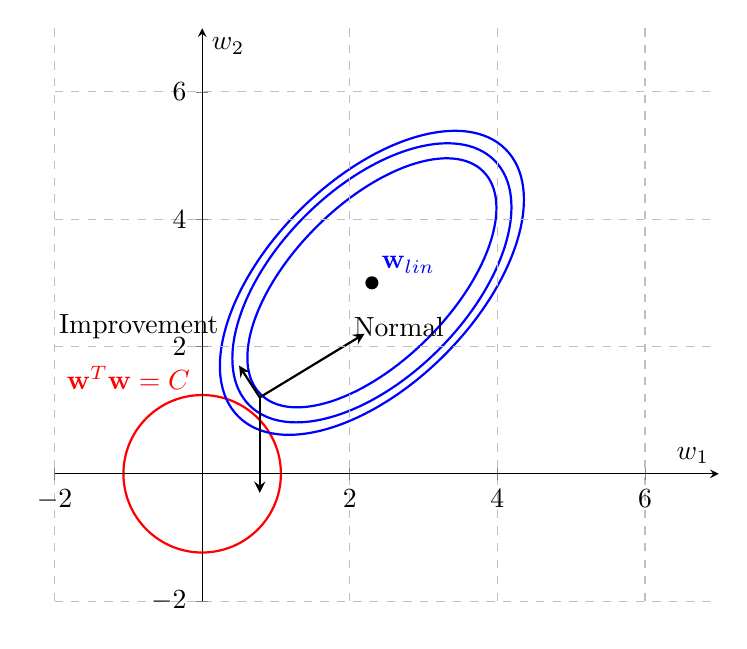
\begin{tikzpicture}
        \begin{axis}[
            xmin=-2, xmax=7,
            ymin=-2, ymax=7,
            axis lines=center,
            axis on top=true,
            ylabel=$w_2$,
            xlabel=$w_1$,
            domain=-3:6,
            grid=major,
            grid style=dashed,
            scale only axis,
        ]

        % Red circle for the constraint w^Tw = C
        \draw[style=thick, red] (axis cs:0,0) circle [radius=1cm];
        \node[red] at (axis cs:-1,1.5) {$\mathbf{w}^T\mathbf{w} = C$};

        % Blue ellipses for the ridge regression loss contours
        \draw[rotate around={-45:(axis cs:2.3,3)}, blue, thick] (axis cs:2.3,3) ellipse (1cm and 2.0cm);
        \draw[rotate around={-45:(axis cs:2.3,3)}, blue, thick] (axis cs:2.3,3) ellipse (1.2cm and 2.2cm);
        \draw[rotate around={-45:(axis cs:2.3,3)}, blue, thick] (axis cs:2.3,3) ellipse (1.3cm and 2.4cm);

        % Label for w_lin
        \node[anchor=south west, blue] at (axis cs:2.3,3) {$\mathbf{w}_{\text{lin}}$};
        % Point marker for w_lin
        \node[circle, scale=0.5, fill=black] at (axis cs:2.3,3) {};

        % Arrows
        \draw[-stealth, thick] (axis cs:0.78,1.2) -- (axis cs:0.5,1.7) node[pos=1.5, above left] {Improvement};
        \draw[-stealth, thick] (axis cs:0.78,1.2) -- (axis cs:0.78,-0.3);
        \draw[-stealth, thick] (axis cs:0.78,1.2) -- (axis cs:2.2,2.2) node[pos=0.8, above right] {Normal};

        \end{axis}
    \end{tikzpicture}
    \caption{Ridge regression visualisation}
    \label{fig:ridge-regress-viz}
\end{figure}


\begin{figure}[H]
    \centering
    \includegraphics[width=1\linewidth]{img/reg_legendre.png}
    \caption{Fitting Legendre polynomials to the objective function: setting $\lambda$ will affect the outcome of overfitting or underfitting.}
    \label{fig:reg-legendre}
\end{figure}

\subsubsection*{Choosing the Regularisation Parameter \( \lambda \)}
The choice of the regularisation parameter \( \lambda \) plays a critical role in the performance of the regularised model. It controls the trade-off between the fit of the model to the data and the magnitude of the coefficients:

\begin{itemize}
    \item A too-small \( \lambda \) may lead to overfitting, where the model captures noise in the training data.
    \item A too-large \( \lambda \) may lead to underfitting, where the model fails to capture the underlying trend in the data.
\end{itemize}

The value of \( \lambda \) is typically determined through cross-validation.

\subsection{Tikhonov Regularisation}

Tikhonov regularisation introduces a generalisation of the \( L_2 \) norm by allowing for the possibility of non-identity transformation matrices that can encode different types of prior knowledge about the weight coefficients. This general form is given as:

\begin{equation}
\|\mathbf{w}\|_{\Gamma}^2 = \mathbf{w}^T\Gamma^T\Gamma\mathbf{w},
\end{equation}
where \( \Gamma \) is a matrix that can incorporate information about the relationships between different features or can be used to impose specific structures on the solution.

\subsubsection*{Example of Tikhonov Regularisation}
A common choice for \( \Gamma \) is to use a diagonal matrix where the diagonal elements \( \gamma_q \) correspond to the inverse of the variance of each feature, normalising the features with respect to their scale. This choice of \( \Gamma \) leads to a standardised regularisation effect across all features.

\subsection{Lasso L1 Regularisation}

Lasso, which stands for Least Absolute Shrinkage and Selection Operator, is a regularisation technique that employs the \( L_1 \) norm of the weight vector:

\begin{equation}
\|\mathbf{w}\|_1 = \sum_{j=1}^{d} |w_j|,
\end{equation}
where \( d \) is the number of dimensions or features.

\subsubsection*{Lasso Formulation}
The Lasso problem to minimise empirical risk $\widehat{R})n$ can be formulated as:

\begin{definitionbox}{Lasso Problem}
    \begin{equation}
\min_{\mathbf{w}} \underbrace{\left\{ \frac{1}{n} \|\mathbf{Zw} - \mathbf{y}\|^2 \right\}}_{\widehat R_n=\frac1n(Z\mathbf{w}-\mathbf{y})^\top(Z\mathbf{w}-\mathbf{y})} \quad \text{subject to} \quad \|\mathbf{w}\|_1 \leq C,
\end{equation}
where \( C \) is a constant that controls the strength of the regularisation.
\end{definitionbox}



\begin{figure}[H]
    \centering
    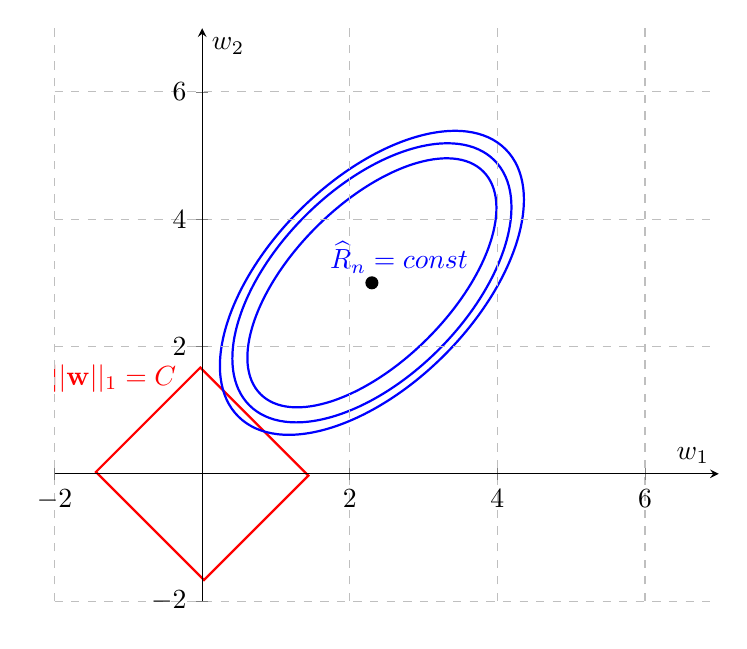
\begin{tikzpicture}
        \begin{axis}[
            xmin=-2, xmax=7,
            ymin=-2, ymax=7,
            axis lines=center,
            axis on top=true,
            ylabel=$w_2$,
            xlabel=$w_1$,
            domain=-3:6,
            grid=major,
            grid style=dashed,
            scale only axis,
        ]

        % Red circle for the constraint w^Tw = C
        \draw[style=thick, red, rotate around={45:(axis cs:0,0)}] (axis cs:-1,-1.2
        ) rectangle (axis cs:1,1.2);
        \node[red] at (axis cs:-1.2,1.5) {$||\mathbf{w}||_1 = C$};

        % Blue ellipses for the ridge regression loss contours
        \draw[rotate around={-45:(axis cs:2.3,3)}, blue, thick] (axis cs:2.3,3) ellipse (1cm and 2.0cm);
        \draw[rotate around={-45:(axis cs:2.3,3)}, blue, thick] (axis cs:2.3,3) ellipse (1.2cm and 2.2cm);
        \draw[rotate around={-45:(axis cs:2.3,3)}, blue, thick] (axis cs:2.3,3) ellipse (1.3cm and 2.4cm);

        % Label for R_n
        \node[anchor=south west, blue] at (axis cs:1.6,3) {$\widehat{R}_{n} = const$};
        % Point marker for w_lin
        \node[circle, scale=0.5, fill=black] at (axis cs:2.3,3) {};

        % Arrows
        % \draw[-stealth, thick] (axis cs:0.78,1.2) -- (axis cs:0.5,1.7) node[pos=1.5, above left] {Improvement};
        % \draw[-stealth, thick] (axis cs:0.78,1.2) -- (axis cs:0.78,-0.3);
        % \draw[-stealth, thick] (axis cs:0.78,1.2) -- (axis cs:2.2,2.2) node[pos=0.8, above right] {Normal};

        \end{axis}
    \end{tikzpicture}
    \caption{Lasso regression visualisation}
    \label{fig:lasso-regress-viz}
\end{figure}

\subsubsection*{Lasso Regularisation}
Lasso (Least Absolute Shrinkage and Selection Operator) employs \( L_1 \) penalty to achieve sparse solutions, effectively performing feature selection by constraining the sum of the absolute values of the model coefficients. This approach is beneficial in high-dimensional spaces where \( d \approx n \) or \( d > n \), as it reduces model complexity and prevents overfitting by enforcing some coefficients to shrink to zero. 


\begin{sidenotebox}{More information on the L1 Norms in Regularisation and why not the L0 Norm \\ }
\subsubsection*{The Problem}
We want to drop out features (components in the weight vector) that we don't need to make things sparse. So we want to minimise the number of non-zero weights in our weight vector.\\

Naively, we could start by constraining the $L_0$-Norm (mathematically, this isn't an actual norm):

\begin{equation*}
\|\mathbf{w}\|_0=\sum_{j=1}^d\mathbb{I}\left(\mathbf{w}_i\neq0\right)
\end{equation*}

Where $\mathbb{I}$ is the indicator function that returns 1 if the condition in its input is true, and 0 otherwise. So this is just the summation of all non-zero weights of the vector $\mathbf{w}$. However, this is a non-convex and NP-hard problem – there is no algorithm that can search through all possible subsets of features, this is a combinatorial search problem in $O(2^d)$ where $d$ is the number of features.\\

Instead, we set the constraint to be the $L_1$ norm of weights:

\[\|\mathbf{w}\|_1=\sum_{j=1}^d|\mathbf{w}_j|\]


Instead of going through all subsets of choosing weights or dropping them, we just set a  simpler limit on their absolute sum. This is a convex optimisation problem that can be solved more efficiently. In Figure \ref{fig:lasso-regress-viz}, note that the $L_1$ norm still is able to shrink coefficients exactly to zero, unlike the $L_2$ norm. This occurs because the optimisation function's contour lines are sharp around the axes where they intersect the elliptical contour of the empirical risk or loss function. At this point, we see that one coefficient on the axis is zero. All optimal values lie precisely on the axis. This is because the $L_1$ norm is shaped more like a diamond than a circle like in $L_2$ regularisation.\\

    However, the $L_1$ norm introduces some bias into the estimates, when true weights values are large. This happens because it shrinks all coefficients towards zero by the same absolute amount, not just the less significant ones – it does not consider true magnitude of each weight.\\
    
    Also, unlike it does not guarantee the selection of the correct subset of features all the time, especially when features are correlated.
\end{sidenotebox}

\subsubsection*{Mathematical Formulation}
The optimisation problem for Lasso is given by the Langrangian, combining the risk function as our objective, plus a multiple of the constraint:
\begin{equation}
\min_{\mathbf{w}} \left\{ \hat{R}_n(\mathbf{w}) + \lambda \|\mathbf{w}\|_1 \right\},
\end{equation}
where \( \hat{R}_n(\mathbf{w}) \) represents the empirical risk and \( \|\mathbf{w}\|_1 = \sum_{j=1}^{d} |\mathbf{w}_j| \) is the \( L_1 \) norm imposing sparsity. The parameter \( \lambda \) controls the degree of sparsity.

% \subsubsection*{Geometrical Insight}
% The \( L_1 \) norm's diamond contour interacts with the elliptical contours of the loss function, frequently intersecting at axes which correspond to sparser solutions. The intersection points represent feature selection through coefficient elimination.


% \subsubsection*{Lasso Constraint Selection}
% The key characteristic of Lasso regularisation is its ability to perform feature selection. The \( L_1 \) penalty has the property of forcing some coefficients to be exactly zero when the regularisation parameter \( \lambda \) is sufficiently large. This leads to models that are sparse with respect to the features used, providing an intrinsic method for feature selection.

% \subsubsection*{Sparse Solutions}
% The geometry of the \( L_1 \) penalty function makes it more likely that the optimisation path will hit the axes in the parameter space, which corresponds to a solution where some of the weights are exactly zero. This is illustrated in the contour plot where the elliptical contours of the loss function intersect with the diamond-shaped contours of the \( L_1 \) norm.

\subsubsection*{Sparse Models and Overfitting}
Sparse models are particularly useful in situations where the number of features \( d \) is close to or greater than the number of samples \( n \). By reducing the number of features, Lasso helps to mitigate the risk of overfitting, which can be a significant concern in high-dimensional datasets.


\subsubsection*{Benefits of LASSO Over Ridge}
LASSO has the advantage of producing sparse models, where some of the coefficients can become exactly zero, thereby performing feature selection:

\begin{itemize}
    \item This sparsity can be beneficial in high-dimensional datasets where it is desirable to reduce the number of features.
    \item It can lead to simpler models that are easier to interpret.
\end{itemize}

\begin{sidenotebox}{Elastic Net Regularisation}
Elastic Net is a compromise between ridge regression and LASSO, combining the \( L_2 \) penalty of ridge regression with the \( L_1 \) penalty of LASSO. It is useful when there are multiple features that are correlated with one another.

\begin{definitionbox}{Elastic Net Regularisation}
The regularisation term for Elastic Net is a linear combination of the \( L_1 \) and \( L_2 \) penalties:
\[
\lambda \left( \alpha \|\mathbf{w}\|_1 + \frac{1-\alpha}{2} \|\mathbf{w}\|_2^2 \right)
\]
where \( \alpha \) is the mixing parameter between \( L_1 \) penalty (LASSO) and \( L_2 \) penalty (ridge), typically chosen via cross-validation.
\end{definitionbox}

\subsubsection*{Algorithmic Implications}
The choice between ridge, LASSO, and Elastic Net also has algorithmic implications:

\begin{itemize}
    \item Ridge regression has a closed-form solution, which can be computed efficiently even for large datasets.
    \item LASSO and Elastic Net may require iterative methods to find a solution, which can be computationally more intensive.
\end{itemize}

The computational complexity should be considered when choosing the regularisation method, especially for large-scale applications.

\subsubsection*{Regularisation in Non-Linear Models}
While regularisation is commonly discussed in the context of linear models, it is equally applicable to non-linear models:

\begin{itemize}
    \item In kernel methods, regularisation controls the complexity of the model in the high-dimensional feature space induced by the kernel.
    \item In neural networks, regularisation can take various forms, including weight decay (similar to \( L_2 \) regularisation) and dropout (a form of stochastic regularisation).
\end{itemize}
\end{sidenotebox}

\subsection{Tikhonov Regularisation}

Tikhonov regularisation is applied in the context of machine learning to prevent overfitting and to improve the generalisation of the model. It does this by adding a regularisation term to the loss function, which penalises complex models:

\begin{itemize}
    \item The loss function with Tikhonov regularisation is given by:
    \[
    \mathcal{L}_n(\mathbf{w}) = \hat{R}_n(\mathbf{w}) + \lambda \|\mathbf{w}\|_Q^2,
    \]
    where \( \hat{R}_n(\mathbf{w}) \) is the empirical risk, \( \lambda \) is the regularisation parameter, and \( \|\mathbf{w}\|_Q^2 \) is the Tikhonov regulariser.
    
    \item The Tikhonov regulariser can be expressed as a weighted sum of the squared weights:
    \[
    \|\mathbf{w}\|_Q^2 = \sum_{q=0}^{Q} \gamma_q w_q^2,
    \]
    where \( \gamma_q \) are the weights that can be adjusted to control the regularisation of the corresponding parameters \( w_q \).

    \item The regularisation term places emphasis on certain weights, which can be tuned according to the desired complexity of the model:
    \begin{itemize}
        \item For a low-order fit, which favours simplicity, the weights \( \gamma_q \) can be chosen as \( \gamma_q = 2^q \).
        \item For a high-order fit, which allows for more complexity, the weights \( \gamma_q \) can be chosen as \( \gamma_q = 2^{-q} \).
    \end{itemize}
\end{itemize}

Tikhonov regularisation introduces a generalisation of the \( L_2 \) norm by allowing for the possibility of non-identity transformation matrices that can encode different types of prior knowledge about the weight coefficients. This general form is given as:



\begin{equation}
\|\mathbf{w}\|_{Q}^2 = \mathbf{w}^T\Gamma^T\Gamma\mathbf{w} \quad Q = \Gamma^\top\Gamma,
\end{equation}
where \( \Gamma \) is a matrix that can incorporate information about the relationships between different features or can be used to impose specific structures on the solution.

\subsubsection*{Example of Tikhonov Regularisation}
A common choice for \( \Gamma \) is to use a diagonal matrix where the diagonal elements \( \gamma_q \) correspond to the inverse of the variance of each feature, normalising the features with respect to their scale. This choice of \( \Gamma \) leads to a standardised regularisation effect across all features.




\section{The Need for Validation}
\subsection*{Example Problem}
\begin{figure}[H]
    \centering\includegraphics[width=0.75\linewidth]{img/choose_lambda.png}
    \caption{If we have too much deterministic and stochastic noise, this increases our chance of overfitting. Increasing the number of data points and our regularisation coefficient $\lambda$ helps to combat this.}
    \label{fig:enter-label}
\end{figure}

\subsection*{Regularised Loss Function}
The regularised loss, denoted as \( L_n(h) \), combines the empirical risk \( \hat{R}(h) \) with a regularisation term \( \Omega(h) \), scaled by a factor \( \lambda \):
\begin{equation}
  L_n(h) = \hat{R}(h) + \lambda \underbrace{\Omega(h)}_{\text{overfit penalty (regularisation)}}
\end{equation}
where \( \lambda \) is the regularisation coefficient controlling the trade-off between the empirical risk and the penalty term.\\

Note the similarity in structure to the Vapnik-Chervonenkis (VC) inequality provides a theoretical bound on the model's generalisation error:
\begin{equation}
  R(h) \leq \hat{R}(h) + \underbrace{\Omega(n, H, \delta)}_{\text{complexity penalty}}
\end{equation}
where \( \Omega(n, H, \sigma) \) represents the complexity penalty associated with the hypothesis space \( H \), the sample size \( n \), and the variance \( \sigma \) of the noise in the data.\\

In essence, we ideally want to minimise the true risk $R(h)$. However, due to limited knowledge, data, noise, true distribution, etc, we cannot compute true risk directly.\\

In earlier section \ref{vc-ineq-subsection} we learnt the VC inequality provides a theoretical upper bound on the true risk based on empirical risk plus a complexity term that depends on the number of data samples $n$, capacity of hypothesis space $\mathcal{H}$, and confidence level $\delta$. \\

In regularisation, we add a penalty term $\Omega (h)$ as an attempt to approximate the complexity term in the VC inequality, by penalising the model complexity we ensure we do not overfit to training data, which is aligned with the goal of VC inequality to control true risk.\\

\begin{commentbox}{Note to Self}
    \textbf{NOTE: the module slides says that $\mathcal{L}_n(h)$ approximates true risk better than the VC inequality, this needs further checking.}
\end{commentbox}


\subsection*{Types of Regularisers}
Various regularisation techniques are used to control different aspects of model complexity:
\begin{itemize}
  \item Ridge Regression: \( \|\mathbf{w}\|_2^2 \) penalises the square of the coefficients, favouring smaller, more diffuse weight values.
  \item Lasso: \( \|\mathbf{w}\|_1 \) encourages sparsity in the model's coefficients, leading to feature selection.
  \item Elastic Net: \( \|\mathbf{w}\|_1 + \|\mathbf{w}\|_2^2 \) combines the penalties of ridge regression and lasso, balancing between feature selection and coefficient shrinkage.
  \item Tikhonov Regularisation: \( \mathbf{w}^T\mathbf{Q}\mathbf{w} \) allows incorporation of prior knowledge through matrix \( \mathbf{Q} = \Gamma^\top \Gamma \) where $\Gamma$ is a matrix of weights.
\end{itemize}


\subsection*{Occam's Razor and Regularisation}
Occam's razor posits that simpler explanations are generally preferable, so in machine learning, we tend to choose simpler models when regularising.\\

This is because noise, which is inherently present in data, is not smooth or structured; therefore, a smoother function, less likely to capture noise, is more desirable.
Validation is a critical process in the development of a machine learning model. It allows for the evaluation of the model's performance on an independent data set, known as the validation set. The following steps outline the validation process in both specific and general contexts, incorporating regularization, hypothesis classes, and the selection of hyperparameters.

\section{Validation}
Regularisation involves adding an overfit penalty to the empirical risk, to determine the final performance.
\[\mathcal{L}_n(h)=\widehat{R}_n(h)+\lambda\underbrace{\Omega(h)}_{\text{overfit penalty}}\]

Validation is attempt to directly estimate the performance by training the model on a portion of the dataset and using another unseen portion of data to gauge its performance.
\[\underbrace{\mathcal{L}_n(h)}_{\text{direct estimation}}=\widehat{R}_n(h)+\lambda\underbrace{\Omega(h)}_{\text{overfit penalty}}\]

\subsection*{Validation Process}
In this section, $n$ refers to the size of the whole dataset and $v$ refers to the size of the validation dataset.
\begin{enumerate}
  \item Split the training data \( D \) into training \( D_{\text{train}} \) and validation \( D_{\text{val}} \) sets.
  \item Train the model \( g \) on \( D_{\text{train}} \).
  \item Estimate its performance on \( D_{\text{val}} \) with \( v = |D_{\text{val}}| \):
  \begin{equation}
    \check{R}_{v}(g) = \frac{1}{v} \sum_{(x,y) \in D_{\text{val}}} \ell(g(x), y)
  \end{equation}
  where \( \ell(g(x), y) \) is the loss function evaluating the prediction \( g(x) \) against the true output \( y \).
  \item Utilise the validation set to provide an unbiased estimate of the true risk \( R(g) \), which, under certain conditions, is very close to the expected risk calculated through validation \[\mathbb{E}_{\mathcal{D}_{\mathrm{val}}}\left[\check{R}_{\nu}(\mathbf{g})\right]\approx R(\mathbf{g})\leqslant\quad\check{R}_{\nu}(\mathbf{g})+\underbrace{\Omega(\mathbf{v},\mathbf{\delta})}_{\sim\sqrt{\log(1/\delta)/v}\leftarrow\text{one model only on }\mathbf{v}-\mathrm{points}} \text{with probability }1-\delta \]
\end{enumerate}

The validation dataset \( D_{\text{val}} \) is unbiased, with a small Hoeffding bound, and only one hypothesis \( g \) is considered.
Select \( \lambda^* \) as the argument that minimises the regularised risk \( \hat{R}_{\lambda}(g) \),
\begin{equation*}
    \lambda^* = \underset{\lambda}{\mathrm{argmin}} \, \hat{R}_{\lambda}(g),
\end{equation*}
then train on the whole dataset \( D \) with \( \lambda^* \).


\subsection*{Validation More Generally}

\begin{enumerate}
  \item Given hypothesis classes \( (\mathcal{H}_1, \lambda_1), \ldots, (\mathcal{H}_m, \lambda_m) \), split \( D \) into \( D_{\text{train}} \) and \( D_{\text{val}} \).
  \item Train \( g_i \) on \( D_{\text{train}} \) with \( |D_{\text{train}}| = n - v \), where $n$ is the size of the whole dataset and $v$ is the size of the validation dataset.
  \item Select \( i_* \) such that \( g_i* = \arg\min_{g_i} \hat{R}_{\text{v}}(g_i) \) on \( |D_{\text{val}}| = v \), where \( i \) can represent not only regularisation but also other hyperparameters.
  \item Select \( \mathcal{H}_i, \lambda_i \) and train new \( g \) on \( D_{\text{val}} \cup D_{\text{train}} \) to get the final \( g^* \).
\end{enumerate}

\begin{figure}[H]
    \centering
    \includegraphics[width=0.75\linewidth]{img/validation.png}
    \caption{Credit: Caltech ML Lectures}
    
\end{figure}


Note that as you increase your validation set size, you will end up picking a hypothesis that best matches the actual true risk for that hypothesis $R(h)$ (denoted as $E_{out}$), however, this error is expected to be higher, a compromise that comes with shrinking the training set size because you increased the validation set size.

\begin{figure}[H]
    \centering
    \includegraphics[width=0.5\linewidth]{img/bias_validation.png}
    \caption{Credit: Caltech ML Lectures}
    
\end{figure}

\subsection*{Discussion and Considerations}

\begin{itemize}
  \item The choice of \( v \) influences the bias-variance trade-off. A small \( v \) may lead to an underestimate of the true risk, while a large \( v \) may increase the variance of the risk estimate.
  \item The size of \( D_{\text{val}} \) is often set to \( \frac{|D|}{5} \) as a rule of thumb, balancing the need for a representative validation set against the need to retain sufficient training data.
  \item Note: the terminology here calls this the "validation set" as opposed to "test set", to emphasise the iterative nature of model selection, which may involve multiple rounds of training and validation before a final test on an unseen data set.
\end{itemize}

\subsection{K-Fold Cross-Validation}
\begin{figure}[H]
    \centering
    \includegraphics[width=0.5\linewidth]{img/crossv.png}
    \caption{Cross Validation illustrated, the red cells refer to the validation subsets}
    \label{fig:crossv}
    % \caption{Enter Caption}
    
\end{figure}
K-fold cross-validation is a model validation technique to assess the predictive performance of a machine learning model. It helps ensure that the model's performance is independent of the way we partition the data into training and test sets.\\

This involves fitting and evaluating $K$ models, training on a (usually larger) set of data and validating on a (usually smaller) portion of unseen data, as seen in Figure \ref{fig:crossv}

\subsection*{Procedure}
Given a dataset $\mathcal{D}$ and a hypothesis class $\mathcal{H}$ with hyperparameter $\theta$, the K-fold cross-validation process is as follows:

\begin{enumerate}
    \item Partition the dataset $\mathcal{D}$ into $K$ distinct subsets $\mathcal{D}_1, \mathcal{D}_2, \ldots, \mathcal{D}_K$ of equal size. Each subset $\mathcal{D}_k$ serves as a validation set, and the remaining $K-1$ subsets are used as the training set.
    
    \item For each hypothesis $(\mathcal{H}_i, \theta_i)$ in the hypothesis classes $(\mathcal{H}_1,\theta_1),(\mathcal{H}_2,\theta_2),\ldots,(\mathcal{H}_M,\theta_M)$, repeat the following steps:
    \begin{enumerate}
        \item Train a model $g_i$ using empirical risk minimization (ERM) on the training set excluding $\mathcal{D}_k$.
        \item Evaluate the validation error $R_{\mathcal{V}}(g_i)$ of the model $g_i$ on the validation set $\mathcal{D}_k$.
        \item Select the model $g_{i^*} = \arg\min_{g_i} R_{\mathcal{V}}(g_i)$ with the lowest validation error.
    \end{enumerate}
    
    \item After training and evaluating on all $K$ folds, use the hypothesis $(\mathcal{H}_{i^*}, \theta_{i^*})$ and the entire dataset $\mathcal{D}$ to train the final model $g^*$.
\end{enumerate}

Example: If you use $K=3$, you would find the best model $g$ that is trained on subset 1 and 2 and validated on 3. Then find the best model trained on 2, validated on 1 and 3. Then find the best model trained on 3, validated on 1 and 2.Then take the average of the cross-validation error for all three cases, this will be an estimate for expected generalisation error.

\subsection*{Mathematics of K-fold Cross Validation}
The validation error $R_k(g_{i_k})$ for each fold $k$ is calculated as:
\begin{equation}
\check{R}_k(g_{\bar{k}})=\frac{1}{|\mathcal{D}_k|}\sum_{(\mathbf{x}_i,\mathbf{y}_i)\in\mathcal{D}_k}\ell(g_{\bar{k}}(\mathbf{x}_i),y_i)\quad \text{ with }\bar{n}=(K-1/K)n
\end{equation}
where $\ell$ is the loss function, $(x_i, y_i)$ are the data points in the validation set $\mathcal{D}_k$, and $|\mathcal{D}_k|$ is the size of the validation set.

The cross-validation error $R_{\text{CV}}$ is the average of the validation errors over all $K$ folds:
\begin{equation}
R_{\text{CV}} = \frac{1}{K} \sum_{k=1}^{K} R_k(g_{i_k})
\end{equation}

The expected cross-validation error is an unbiased estimate of the expected generalisation error:
\begin{equation}
\mathbb{E}_{\mathcal{D}} [R_{\text{CV}}] = \mathbb{E}_{\mathcal{D}} [R(g_{i_k})]
\end{equation}

\subsection*{Typical Choices for \textit{K}}
\begin{itemize}
    \item $K = 10$: This is the standard choice for 10-fold cross-validation.
    \item $K = n$: Known as leave-one-out cross-validation, where $n$ is the number of data points in the dataset $\mathcal{D}$ This is usually done when there is a small dataset and the model is not too computationally expensive, because this requires a lot of training iterations, creating and evaluating one model for each example in the dataset.
\end{itemize}

\section{Revisiting The SRM}

We have covered Structural Risk Minimisation and Validation previously in \ref{SRM-section}:

\begin{definitionbox}{Structural Risk Minimisation}


From the generalisation bound of the VC Inequality in
\[R(h) \leq \widehat{R}_n(h) + \sqrt{\frac{8d_{VC}(\mathcal{H})}{n} \log\left(\frac{2n + 1}{\delta}\right) + \frac{8}{n} \log\frac{4}{\delta}}\\\]

We have with probability of at least $1-{\color{red} w_i}\delta$, for all $h \in \mathcal{H}_i$:
    \begin{align*}
R(h) &\leq \widehat{R}_n(h) + \sqrt{\frac{8d_{VC}(\mathcal{H})}{n} \log\left(\frac{2n + 1}{\delta}\right) + \frac{8}{n} \log\frac{4}{w_i\delta}}\\
R(h) &\leq \widehat{R}_n(h) + \Omega(n, \mathcal{H}_i, {\color{red} w_i}\delta)    
    \end{align*}
SRM Solution: 
    \[g = \text{argmin}_{h \in \mathcal{H}}\widehat{R}_n(h) + \Omega(n, \mathcal{H}(h), {\color{red} w_i}\delta)\]

    \begin{itemize}
        \item $\mathcal{H}(h)$ is the simplest class $h$ belongs to, and $w_i$ is the class weight.
        \item Training error $\hat{R}_n(h)$ plus complexity term $\Omega$ (from VC inequality).
        \item Identical to ERM if there is only one class $\mathcal{H}$.
    \end{itemize}

    \end{definitionbox}

    \begin{definitionbox}{Generalisation Bound}
        We then have, with probability of at least $1-\delta$,

        \begin{align*}
R(\mathbf{g})& \leqslant\min_{i}\left(R(h_{i}^{*})+2\Omega(n,{\mathcal H}_{i},w_{i}\delta)\right)  \\
&\leqslant R(h^*)+2\Omega(n,\mathcal{H}(h^*),w(h^*)\delta)
\end{align*}

Where $h^*_i = \text{argmin}_{h\in\mathcal{H}_i}R(h_i)$ and $h^* = \text{argmin}_{h\in\mathcal{H}}R(h)$.\\

This means that our risk for our hypothesis $g$ determined by SRM (which factors in for regularisation penalities) is bounded by the true risk plus the VC inequality complexity penalty for that given hypothesis class.

\subsubsection*{Proof:}
Let $\Omega_h = \Omega(n, \mathcal{H}(h), w(h)\delta)$. Then with probability of at least $1-\delta$ for any $h \in \mathcal{H}:$
\[R(g)-R(h)=\underbrace{R(g)-(\hat{R}_n(g)+\Omega_g)}_{\leqslant0\text{ (VC inequality)}}+\underbrace{(\hat{R}_n(g)+\Omega_g)-(\hat{R}_n(h)+\Omega_h)}_{\leqslant0\text{ by def. of g}}+{\color{red}\Omega_h}+\underbrace{\hat{R}_n(h)-R(h)}_{\leqslant{\color{red}\Omega_h}\text{ (VC inequality)}}\]
    \end{definitionbox}

\subsection*{Hypothesis Space and Preferences}
The hypothesis space \( \mathcal{H} \) is structured as a union of nested classes \( \mathcal{H}_i \), each with an associated complexity and preference weight \( w_i \), with \( \sum w_i = 1 \).

\subsection*{Choosing Weights}
The selection of weights \( w_i \) influences the trade-off between model complexity and fit to the data, akin to selecting a regularization parameter in practical applications. No preference implies equal weighting ($w_i = 1/N$) for $N$ classes, whereas a preference for simplicity implies higher weights for simpler models.


\begin{figure}[H]
    \centering
\includegraphics[width=1\linewidth]{img/RLM.png}
\includegraphics[width=0.75\linewidth]{img/srm-2side.png}    
\includegraphics[width=0.75\linewidth]{img/srm2.png}
\end{figure}

\begin{figure}[H]
    \centering
\includegraphics[width=0.55\linewidth]{img/terminology_3.png}

\end{figure}

\section{Approaching a Practical Machine Learning Problem}

\begin{enumerate}
    \item Take the problem and translate its details into a machine learning problem.
    \begin{itemize}
        \item Identify what kind of task it is, classification, regression, etc.
        \item Convert input data into a vector representation \textbf{x}
        \item Utilise an error or loss function $\ell(h(x),y)$ based on the application.
        \item Select hypothess classes $\mathcal{H}$ with their learning algorithms
    \end{itemize}
    \item Follow one of the know methods: ERM, SRM, Regularisation, Validation
    \item Plan and execute experiments
    \item Present and analyse the results
\end{enumerate}
